% !TEX root = ../../thesis.tex

\section{Numerics}
Proving quantities are conserved is a great way of theoretically verifying our results are correct. However in practicality the reason that numerical analysts are interested in this area of mathematics is to create more precise numerical schemes. We shall now show that normal numerical schemes sometimes provide non-realistic solutions and show how we can produce more realistic results.\\

\noindent
We shall take the standard Euler equations as a simplistic example to show our point. Consider the following Euler equation.
$$ \pd {\vec u} t + ({\vec u} \cdot\nab){\vec u} = 0. $$
We can run a Crank-Nicholson scheme on this. It is well known that Crank-Nicholson is symplectic, that is it preserves the symplectic form. Further, this means that it conserves energy. These schemes can be adapted to conserve other quantities. To motivate these we consider a finite element scheme with a cubed $50\times 50$ grid with order $2$ Lagrange elements. We set an initial condition of,
$$ u_0(x,\, y) = \left( -\cos \left( \frac{\pi x}{2} \right)\sin \left( \frac{\pi x}{2} \right),\, \sin\left( \frac{\pi x}{2} \right)\cos \left( \frac{\pi y}{2} \right) \right), $$
and Neumann boundary conditions. The finite element scheme solves for the spatial steps and we use a Crank-Nicholson for the temporal steps. Hence our scheme is,
$$ \frac{{\vec u}^{n+1} - {\vec u}^n}{\D t} = \frac{1}{2}\left( \left({\vec u}^{n+1} \cdot \nab\right){\vec u}^{n+1} + \left({\vec u}^{n} \cdot \nab\right){\vec u}^{n}\right). $$
This produces the following simulation,
\begin{figure*}
    \centering
    \begin{subfigure}[b]{0.475\textwidth}
        \centering
        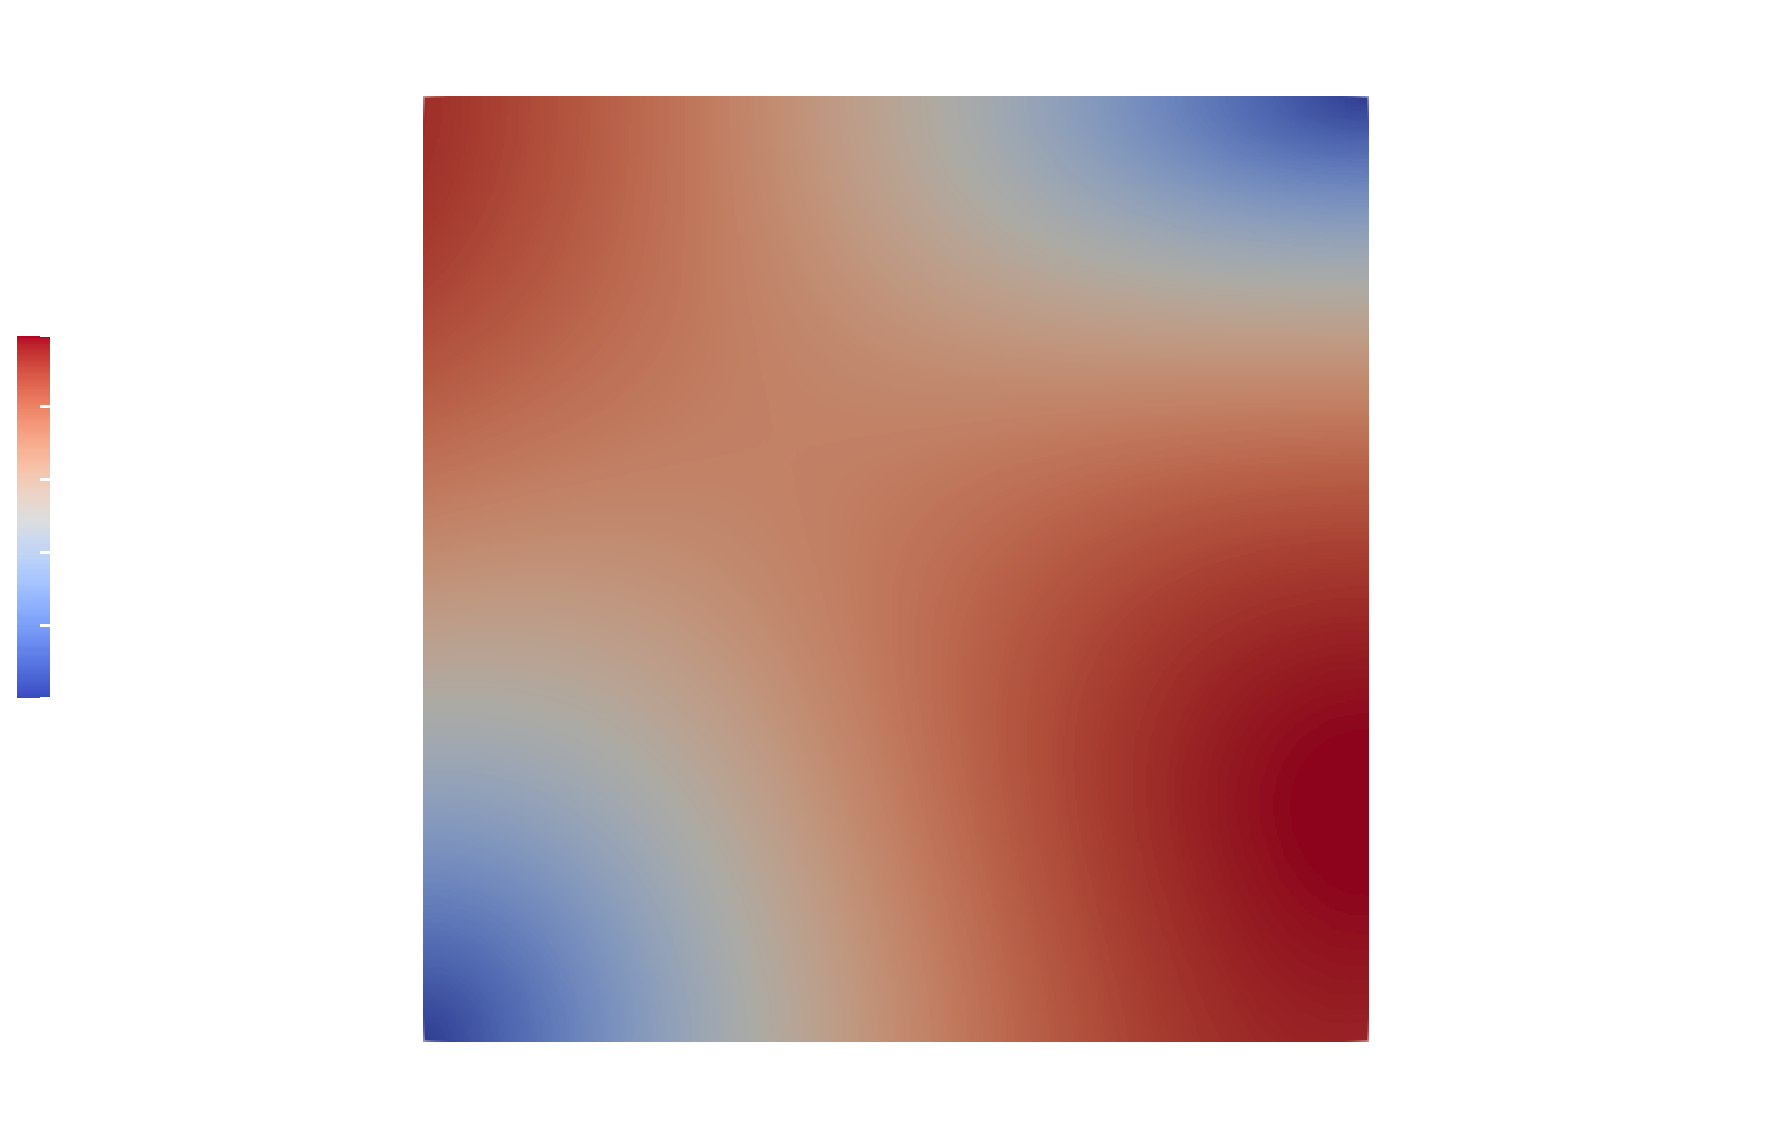
\includegraphics[width=\textwidth]{./img/25.eps}
        \caption[Network2]%
        {{\small Network 1}}
        \label{fig:mean and std of net14}
    \end{subfigure}
    \hfill
    \begin{subfigure}[b]{0.475\textwidth}
        \centering
        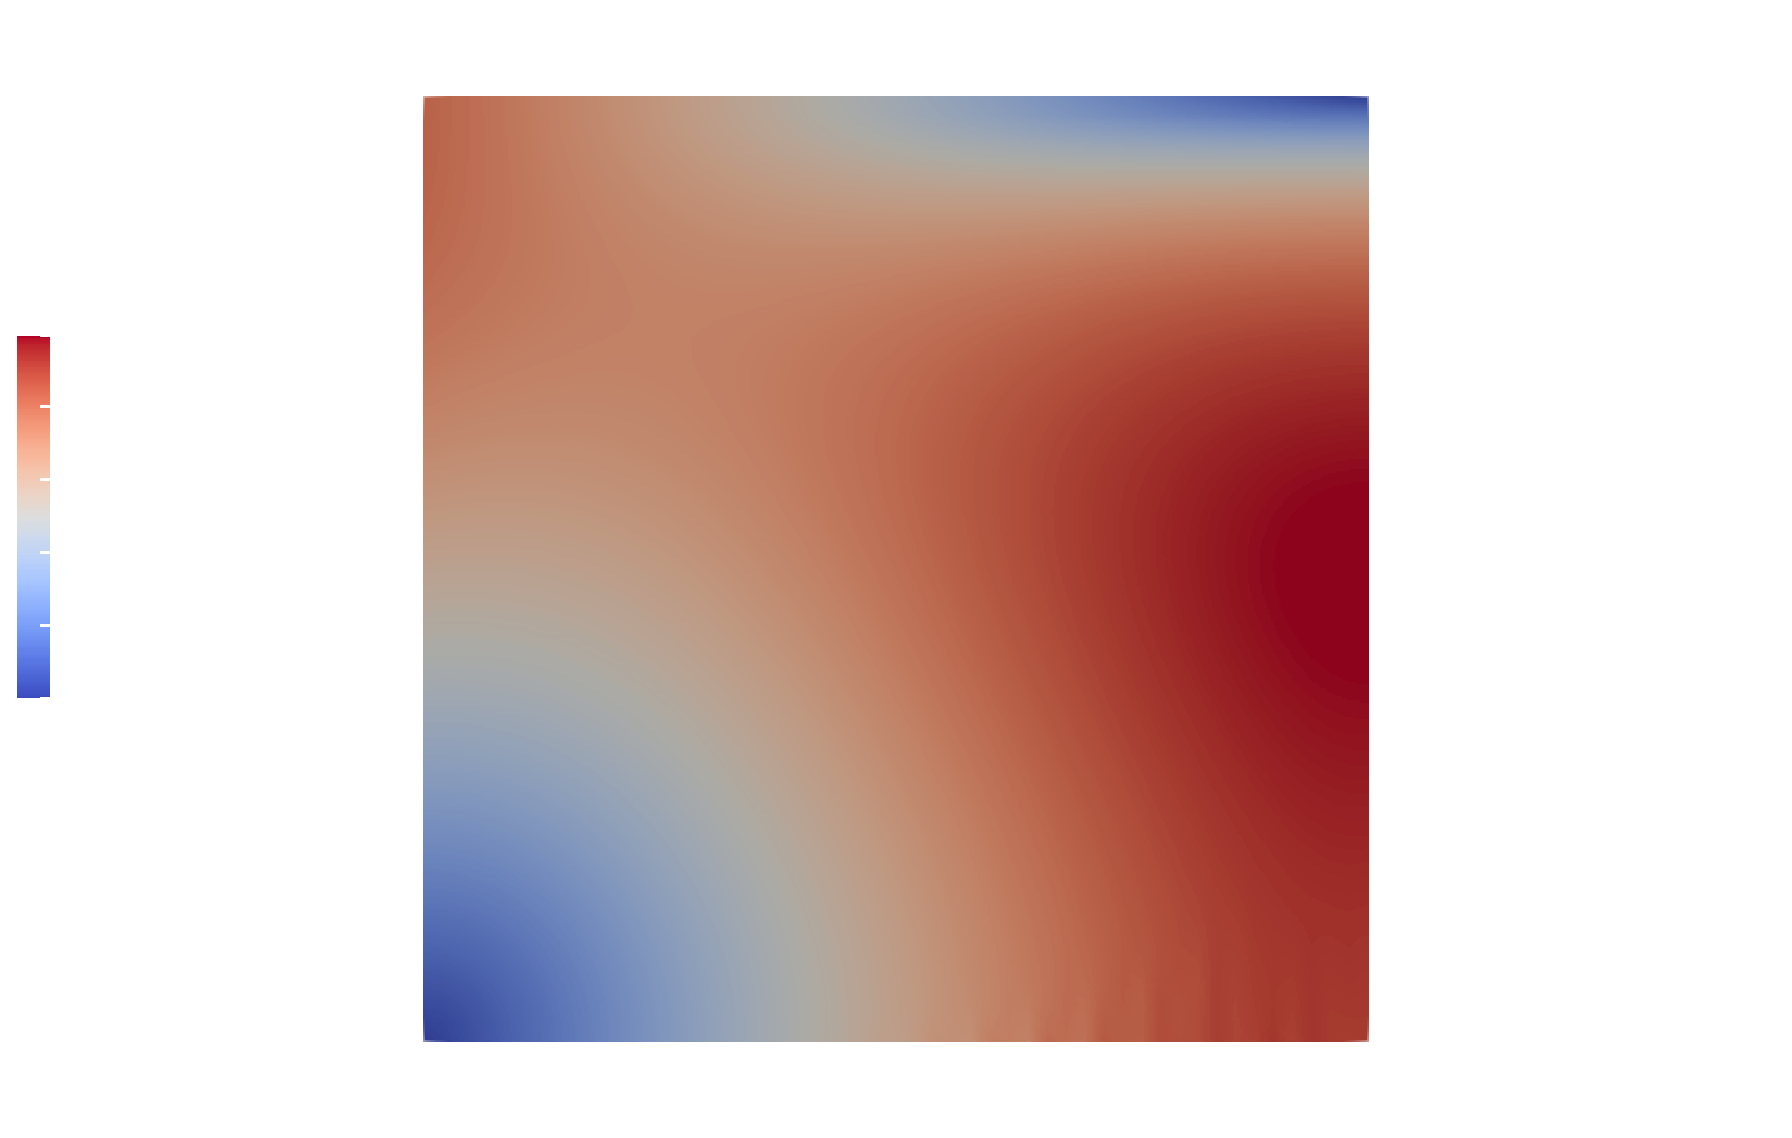
\includegraphics[width=\textwidth]{./img/50.eps}
        \caption[]%
        {{\small Network 2}}
        \label{fig:mean and std of net24}
    \end{subfigure}
    \vskip\baselineskip
    \begin{subfigure}[b]{0.475\textwidth}
        \centering
        \includegraphics[width=\textwidth]{./img/75.eps}
        \caption[]%
        {{\small Network 3}}
        \label{fig:mean and std of net34}
    \end{subfigure}
    \hfill
    \begin{subfigure}[b]{0.475\textwidth}
        \centering
        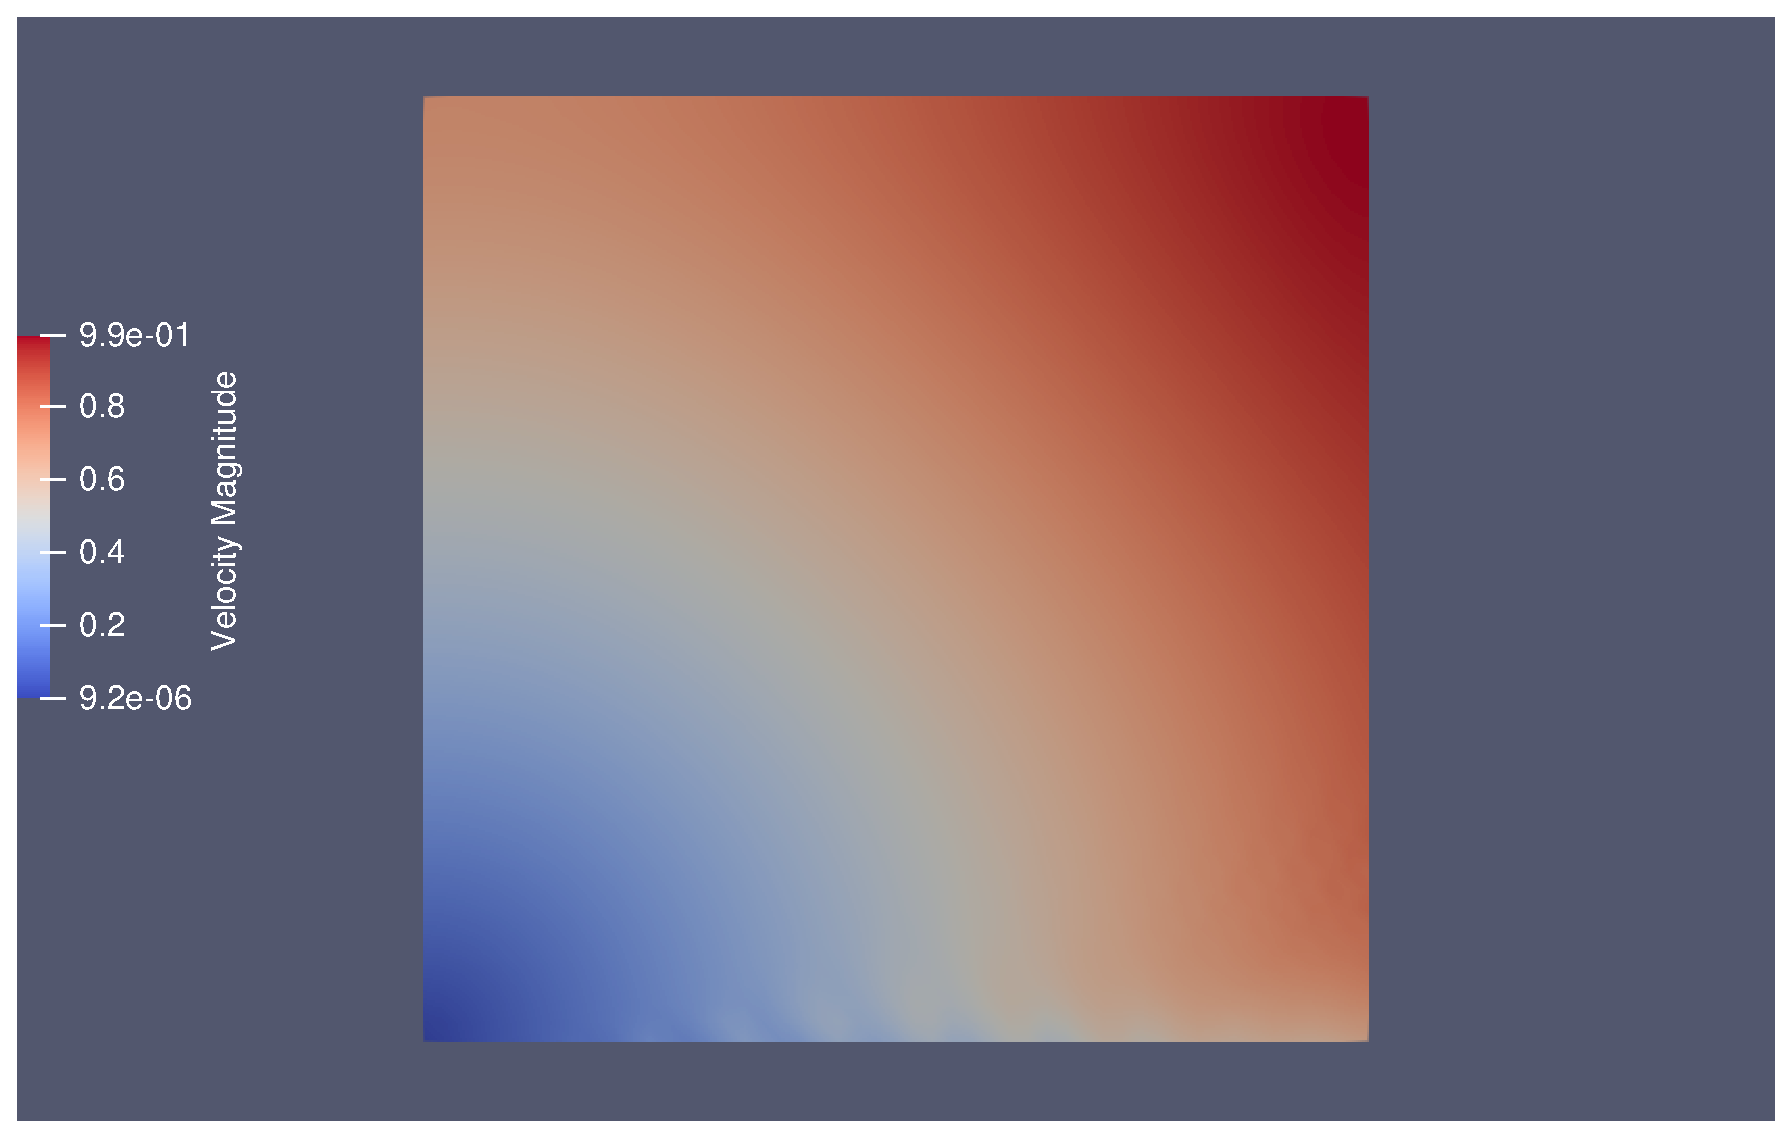
\includegraphics[width=\textwidth]{./img/100.eps}
        \caption[]%
        {{\small Network 4}}
        \label{fig:mean and std of net44}
    \end{subfigure}
    \caption[ The average and standard deviation of critical parameters ]
    {\small The average and standard deviation of critical parameters: Region R4}
    \label{fig:mean and std of nets}
\end{figure*}
